\documentclass[a4paper]{article}
\usepackage[utf8]{inputenc}
\usepackage[spanish, es-tabla, es-noshorthands]{babel}
\usepackage[table,xcdraw]{xcolor}
\usepackage[a4paper, footnotesep=1.25cm, headheight=1.25cm, top=2.54cm, left=2.54cm, bottom=2.54cm, right=2.54cm]{geometry}
%\geometry{showframe}

%\usepackage{wrapfig}			%Wrap figure in text
\usepackage[export]{adjustbox}	%Move images
\usepackage{changepage}			%Move tables

\usepackage{tikz}
\usepackage{amsmath}
\usepackage{amsfonts}
\usepackage{amssymb}
\usepackage{float}
\usepackage{graphicx}
\usepackage{caption}
\usepackage{subcaption}
\usepackage{multicol}
\usepackage{multirow}
\usepackage{wrapfig}
\setlength{\doublerulesep}{\arrayrulewidth}
\usepackage{booktabs}
\usepackage[numbib, nottoc, notlot, notlof]{tocbibind}

\usepackage{hyperref}
\hypersetup{
    colorlinks=true,
    linkcolor=blue,
    filecolor=magenta,      
    urlcolor=blue,
    citecolor=blue,    
}

%Change Font Size

% #1 = size, #2 = text
\newcommand{\setparagraphsize}[2]{{\fontsize{#1}{6}\selectfont#2 \par}}		%Cambia el size de todo el parrafo
\newcommand{\setlinesize}[2]{{\fontsize{#1}{6}\selectfont#2}}				%Cambia el font de una oración

\newcommand{\note}[1]{
	\begin{center}
		\huge{ \textcolor{red}{#1} }
	\end{center}
}

%FONTS (IMPORTANTE): Compilar en XeLaTex o LuaLaTeX
\usepackage{anyfontsize}	%Font size
\usepackage{fontspec}		%Font type

\usepackage{etoolbox}
\usepackage{todonotes}

\newcommand{\observacion}[2]{  \ifnumequal{1}{#1}{ { \todo[inline,backgroundcolor=red!25,bordercolor=red!100]{\textbf{Observación: #2}} } }{  }  }

\setcounter{topnumber}{2}
\setcounter{bottomnumber}{2}
\setcounter{totalnumber}{4}
\renewcommand{\topfraction}{0.85}
\renewcommand{\bottomfraction}{0.85}
\renewcommand{\textfraction}{0.15}
\renewcommand{\floatpagefraction}{0.8}
\renewcommand{\textfraction}{0.1}
\setlength{\floatsep}{5pt plus 2pt minus 2pt}
\setlength{\textfloatsep}{5pt plus 2pt minus 2pt}
\setlength{\intextsep}{5pt plus 2pt minus 2pt}

\newcommand{\quotes}[1]{``#1''}
\usepackage{array}
\newcolumntype{C}[1]{>{\centering\let\newline\\\arraybackslash\hspace{0pt}}m{#1}}
\usepackage[american]{circuitikz}
\usetikzlibrary{calc}
\usepackage{fancyhdr}
\usepackage{units} 

\graphicspath{{../Control de posición no lineal/}{../Control de fuerza no lineal/}{../Control híbrido no lineal/}{../Referencias/}{../Deducción de modelo/}{../Conclusiones/}}

\pagestyle{fancy}
\fancyhf{}
\lhead{22.99 - Automación Industrial}
\rhead{Lambertucci, Londero B., Maselli, Mechoulam}
\rfoot{Página \thepage}

%Items con bullets y no cuadrados
\renewcommand{\labelitemi}{\textbullet }


\begin{document}

\def\verObs{0}

%%%%%%%%%%%%%%%%%%%%%%%%%
%		Caratula		%
%%%%%%%%%%%%%%%%%%%%%%%%%

\setmainfont{AvenirLTStd-Roman}[Path = ./Utils/, Extension = .otf]

\begin{titlepage}

\begin{tikzpicture}[remember picture, overlay, black, line width = 0.5pt]
	\coordinate (a) at (-2cm,2cm);
	\coordinate (b) at (17cm,-25.5cm);
	
	\coordinate (ap) at (-2.1cm,2.1cm);
	\coordinate (bp) at (17.1cm,-25.6cm);
	
	\draw[] (a) -| (b);
	\draw[] (a) |- (b);
	
	\draw[] (ap) -| (bp);
	\draw[] (ap) |- (bp);
	
	%footnotesep=1.25cm, headheight=1.25cm, top=2.54cm, left=2.54cm, bottom=2.54cm, right=2.54cm

\end{tikzpicture}

\begin{figure}[H]
	
\includegraphics[width=0.3\linewidth, right]{./Utils/ITBA_1}
\end{figure}

\vspace*{1.5cm}

\noindent \textbf{\setlinesize{12}{INSTITUTO TECNOLÓGICO DE BUENOS AIRES - ITBA}}

\noindent \textbf{\setlinesize{12}{ESCUELA DE INGENIERÍA Y TECNOLOGÍA}}

\vspace*{4cm}

\begin{center}
	\setlinesize{24}{ \textbf{TRABAJO PRÁCTICO FINAL} }
	
	\vspace*{1.5cm}
	%\setlinesize{24}{ \textbf{Subtítulo del trabajo (cuando corresponda)} }
	\vspace*{1.0cm}
\end{center}
\begin{center}
	\setlinesize{18}{ \textbf{MANUAL DE USUARIO} }
	
	\vspace*{1.5cm}
	%\setlinesize{24}{ \textbf{Subtítulo del trabajo (cuando corresponda)} }
	\vspace*{1.0cm}
\end{center}
\begin{figure}[H]
\begin{adjustwidth}{-1cm}{}
\begin{tabular}{llr} 
	\textbf{AUTORES:}
	& \textbf{Lambertucci, Guido Enrique} & \textbf{(Leg. N}$\mathbf{^o}$ \textbf{58009)} \\
	& \textbf{Londero Bonaparte, Tomás Guillermo} & \textbf{(Leg. N}$\mathbf{^o}$ \textbf{58150)} \\
	& \textbf{Mechoulam, Alan}  &  \textbf{(Leg. N}$\mathbf{^o}$ \textbf{58438)}\\
	& \textbf{Maselli, Carlos Javier} &  \textbf{(Leg. N}$\mathbf{^o}$ \textbf{59564)} \\
	 
 &  & \\
 &  & \\
	\textbf{DOCENTES}:
	& \textbf{Arias, Rodolfo Enrique} & \\
	& \textbf{Sofio Avogadro, Federico} & \\
	& \textbf{Spinelli, Mariano Tomás} & \\
\end{tabular}
\end{adjustwidth}
\end{figure}

\vspace*{0.5cm}
\center{
%{\noindent \setparagraphsize{12}{\textbf{TRABAJO PRÁCTICO N$^{\circ}$1}}}
{\noindent \setparagraphsize{12}{\textbf{\textsc{22.90 - Automación Industrial}}}}
}
\vspace*{1.5cm}

\center{\textbf{BUENOS AIRES}}

\end{titlepage}


\setmainfont{calibri-regular}[Path = ./Utils/, Extension = .ttf, BoldFont=calibrib, ItalicFont=calibrii, BoldItalicFont=calibriz]
\tableofcontents

\newpage

%%%%%%%%%%%%%%%%%%%%%
%		Informe		%
%%%%%%%%%%%%%%%%%%%%%
\Section{Glosario}
%\documentclass[a4paper]{article}
\usepackage[utf8]{inputenc}
\usepackage[spanish, es-tabla, es-noshorthands]{babel}
\usepackage[table,xcdraw]{xcolor}
\usepackage[a4paper, footnotesep=1.25cm, headheight=1.25cm, top=2.54cm, left=2.54cm, bottom=2.54cm, right=2.54cm]{geometry}
%\geometry{showframe}

%\usepackage{wrapfig}			%Wrap figure in text
\usepackage[export]{adjustbox}	%Move images
\usepackage{changepage}			%Move tables

\usepackage{tikz}
\usepackage{amsmath}
\usepackage{amsfonts}
\usepackage{amssymb}
\usepackage{float}
\usepackage{graphicx}
\usepackage{caption}
\usepackage{subcaption}
\usepackage{multicol}
\usepackage{multirow}
\usepackage{wrapfig}
\setlength{\doublerulesep}{\arrayrulewidth}
\usepackage{booktabs}
\usepackage[numbib, nottoc, notlot, notlof]{tocbibind}

\usepackage{hyperref}
\hypersetup{
    colorlinks=true,
    linkcolor=blue,
    filecolor=magenta,      
    urlcolor=blue,
    citecolor=blue,    
}

%Change Font Size

% #1 = size, #2 = text
\newcommand{\setparagraphsize}[2]{{\fontsize{#1}{6}\selectfont#2 \par}}		%Cambia el size de todo el parrafo
\newcommand{\setlinesize}[2]{{\fontsize{#1}{6}\selectfont#2}}				%Cambia el font de una oración

\newcommand{\note}[1]{
	\begin{center}
		\huge{ \textcolor{red}{#1} }
	\end{center}
}

%FONTS (IMPORTANTE): Compilar en XeLaTex o LuaLaTeX
\usepackage{anyfontsize}	%Font size
\usepackage{fontspec}		%Font type

\usepackage{etoolbox}
\usepackage{todonotes}

\newcommand{\observacion}[2]{  \ifnumequal{1}{#1}{ { \todo[inline,backgroundcolor=red!25,bordercolor=red!100]{\textbf{Observación: #2}} } }{  }  }

\setcounter{topnumber}{2}
\setcounter{bottomnumber}{2}
\setcounter{totalnumber}{4}
\renewcommand{\topfraction}{0.85}
\renewcommand{\bottomfraction}{0.85}
\renewcommand{\textfraction}{0.15}
\renewcommand{\floatpagefraction}{0.8}
\renewcommand{\textfraction}{0.1}
\setlength{\floatsep}{5pt plus 2pt minus 2pt}
\setlength{\textfloatsep}{5pt plus 2pt minus 2pt}
\setlength{\intextsep}{5pt plus 2pt minus 2pt}

\newcommand{\quotes}[1]{``#1''}
\usepackage{array}
\newcolumntype{C}[1]{>{\centering\let\newline\\\arraybackslash\hspace{0pt}}m{#1}}
\usepackage[american]{circuitikz}
\usetikzlibrary{calc}
\usepackage{fancyhdr}
\usepackage{units} 

\graphicspath{{../Control de posición no lineal/}{../Control de fuerza no lineal/}{../Control híbrido no lineal/}{../Referencias/}{../Deducción de modelo/}{../Conclusiones/}}

\pagestyle{fancy}
\fancyhf{}
\lhead{22.99 - Automación Industrial}
\rhead{Lambertucci, Londero B., Maselli, Mechoulam}
\rfoot{Página \thepage}

%Items con bullets y no cuadrados
\renewcommand{\labelitemi}{\textbullet }

%
%\begin{document}

\begin{table}[H]
\centering
\begin{tabular}{!{\color{AzulTable}\vrule}ll!{\color{AzulTable}\vrule}}
\arrayrulecolor{AzulTable}
\hline
\rowcolor{AzulTable}
\multicolumn{1}{|l}{\textcolor{white}{Término}} & \multicolumn{1}{l|}{\textcolor{white}{Descripci\'on}} \\ \hline
\textbf{$x_0$}		& \begin{tabular}[l]{@{}l@{}}Posición horizontal del carrito.\end{tabular}							\\ \hline
\textbf{$\theta_1$}		& \begin{tabular}[l]{@{}l@{}}Ángulo entre el primer link con la vertical.\end{tabular}						\\ \hline
\textbf{$\theta_2$}		& \begin{tabular}[l]{@{}l@{}}Ángulo entre el segundo link con la vertical.\end{tabular}						\\ \hline
\textbf{$m_0$}		& \begin{tabular}[l]{@{}l@{}}Masa del carrito.\end{tabular}						\\ \hline
\textbf{$m_1$}		& \begin{tabular}[l]{@{}l@{}}Masa del primer link del péndulo.\end{tabular}						\\ \hline
\textbf{$m_2$}		& \begin{tabular}[l]{@{}l@{}}Masa del segundo link del péndulo..\end{tabular}						\\ \hline
\textbf{$L_1$}		& \begin{tabular}[l]{@{}l@{}}Longitud del primer link.\end{tabular}						\\ \hline
\textbf{$L_2$}		& \begin{tabular}[l]{@{}l@{}}Longitud del segundo link..\end{tabular}						\\ \hline

\textbf{$l_1$}		& \begin{tabular}[l]{@{}l@{}}Distancia entre la base del primer link y su centro de masas.\end{tabular}						\\ \hline

\textbf{$l_2$}		& \begin{tabular}[l]{@{}l@{}}
Distancia entre la base del segundo link y su centro de masas.\end{tabular}						\\ \hline

\textbf{$I_1$}		& \begin{tabular}[l]{@{}l@{}}
Momento de inercia del primer link.
\end{tabular}						\\ \hline

\textbf{$I_2$}		& \begin{tabular}[l]{@{}l@{}}
Momento de inercia del segundo link.
\end{tabular}						\\ \hline

\textbf{$g$}		& \begin{tabular}[l]{@{}l@{}}
Constante de aceleración de la gravedad.
\end{tabular}						\\ \hline

\textbf{$u(t)$}		& \begin{tabular}[l]{@{}l@{}}Acción de Control.\end{tabular}						\\ \hline
\textbf{$\Theta$}		& \begin{tabular}[l]{@{}l@{}}Vector de estados.\end{tabular}						\\ \hline
\textbf{$Y$}		& \begin{tabular}[l]{@{}l@{}}Vector de salida del sistema.\end{tabular}						
\\ \hline
\textbf{$\hat{\Theta}$}		& \begin{tabular}[l]{@{}l@{}}Vector de estados estimado.\end{tabular}						\\ \hline
\textbf{$\hat{Y}$}		& \begin{tabular}[l]{@{}l@{}}Vector de salida del sistema estimado.\end{tabular}						
\\ \hline

\textbf{$\Theta_0$}		& \begin{tabular}[l]{@{}l@{}}Condición Inicial.\end{tabular}						\\ \hline
\textbf{$L$}		& \begin{tabular}[l]{@{}l@{}}Lagrangiano.\end{tabular}						\\ \hline

\textbf{$M\left( \Theta \right)$}		& \begin{tabular}[l]{@{}l@{}}Matriz de influencia de masas/inercia en vector de torques.\end{tabular}						\\ \hline


\textbf{$V\left( \Theta , \dot{\Theta} \right)$}		& \begin{tabular}[l]{@{}l@{}}Vector de influencia de términos centrífugos y de Coriolis.\end{tabular}						\\ \hline

\textbf{$G\left( \Theta \right)$}		& \begin{tabular}[l]{@{}l@{}}Vector de influencia de la gravedad.\end{tabular}						\\ \hline


\end{tabular}
\end{table}
%\end{document}
\newpage
\Section{Resumen}
%\documentclass[a4paper]{article}
\usepackage[utf8]{inputenc}
\usepackage[spanish, es-tabla, es-noshorthands]{babel}
\usepackage[table,xcdraw]{xcolor}
\usepackage[a4paper, footnotesep=1.25cm, headheight=1.25cm, top=2.54cm, left=2.54cm, bottom=2.54cm, right=2.54cm]{geometry}
%\geometry{showframe}

%\usepackage{wrapfig}			%Wrap figure in text
\usepackage[export]{adjustbox}	%Move images
\usepackage{changepage}			%Move tables

\usepackage{tikz}
\usepackage{amsmath}
\usepackage{amsfonts}
\usepackage{amssymb}
\usepackage{float}
\usepackage{graphicx}
\usepackage{caption}
\usepackage{subcaption}
\usepackage{multicol}
\usepackage{multirow}
\usepackage{wrapfig}
\setlength{\doublerulesep}{\arrayrulewidth}
\usepackage{booktabs}
\usepackage[numbib, nottoc, notlot, notlof]{tocbibind}

\usepackage{hyperref}
\hypersetup{
    colorlinks=true,
    linkcolor=blue,
    filecolor=magenta,      
    urlcolor=blue,
    citecolor=blue,    
}

%Change Font Size

% #1 = size, #2 = text
\newcommand{\setparagraphsize}[2]{{\fontsize{#1}{6}\selectfont#2 \par}}		%Cambia el size de todo el parrafo
\newcommand{\setlinesize}[2]{{\fontsize{#1}{6}\selectfont#2}}				%Cambia el font de una oración

\newcommand{\note}[1]{
	\begin{center}
		\huge{ \textcolor{red}{#1} }
	\end{center}
}

%FONTS (IMPORTANTE): Compilar en XeLaTex o LuaLaTeX
\usepackage{anyfontsize}	%Font size
\usepackage{fontspec}		%Font type

\usepackage{etoolbox}
\usepackage{todonotes}

\newcommand{\observacion}[2]{  \ifnumequal{1}{#1}{ { \todo[inline,backgroundcolor=red!25,bordercolor=red!100]{\textbf{Observación: #2}} } }{  }  }

\setcounter{topnumber}{2}
\setcounter{bottomnumber}{2}
\setcounter{totalnumber}{4}
\renewcommand{\topfraction}{0.85}
\renewcommand{\bottomfraction}{0.85}
\renewcommand{\textfraction}{0.15}
\renewcommand{\floatpagefraction}{0.8}
\renewcommand{\textfraction}{0.1}
\setlength{\floatsep}{5pt plus 2pt minus 2pt}
\setlength{\textfloatsep}{5pt plus 2pt minus 2pt}
\setlength{\intextsep}{5pt plus 2pt minus 2pt}

\newcommand{\quotes}[1]{``#1''}
\usepackage{array}
\newcolumntype{C}[1]{>{\centering\let\newline\\\arraybackslash\hspace{0pt}}m{#1}}
\usepackage[american]{circuitikz}
\usetikzlibrary{calc}
\usepackage{fancyhdr}
\usepackage{units} 

\graphicspath{{../Control de posición no lineal/}{../Control de fuerza no lineal/}{../Control híbrido no lineal/}{../Referencias/}{../Deducción de modelo/}{../Conclusiones/}}

\pagestyle{fancy}
\fancyhf{}
\lhead{22.99 - Automación Industrial}
\rhead{Lambertucci, Londero B., Maselli, Mechoulam}
\rfoot{Página \thepage}

%Items con bullets y no cuadrados
\renewcommand{\labelitemi}{\textbullet }

%
%\begin{document}
En el presente trabajo se realiza el control por realimentación de estados tanto integral, para el caso continuo y discreto con observador, para el doble péndulo invertido. 

\begin{figure}[H]
	\centering
	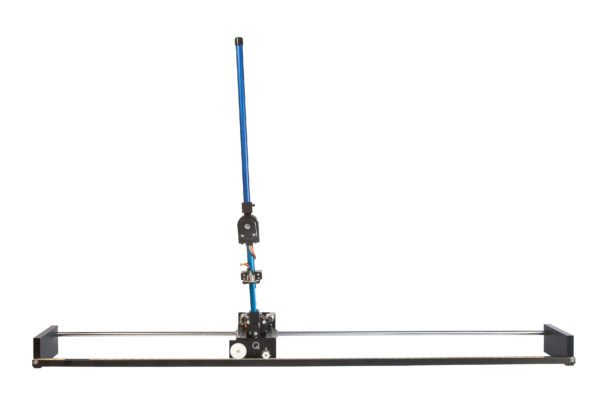
\includegraphics[width=\linewidth]{ImagenesResumen/base}
	\caption{Pendulo doble invertido.}	
	\label{fig:pend}
\end{figure}
Obteniendo el modelo teórico del mismo a partir de ecuaciones, cotejando dicho modelo con los valores linealizados de la planta implementada en Matlab con la ayuda del framework de simscape para su simulación.\\
También se realiza un estudio en las diferencias entre dichos modelos, y entre los distintos resultados de los métodos de control.
\\
Adicionalmente se calcula si el sistema es en efecto controlable y observable, y si existen condiciones en las cuales esto se ve afectado a través del uso de diagramas de Mason.

%\end{document}
\newpage


\Section{Modelo Teórico}
\label{sec:modeloteorico}
%\documentclass[a4paper]{article}
\usepackage[utf8]{inputenc}
\usepackage[spanish, es-tabla, es-noshorthands]{babel}
\usepackage[table,xcdraw]{xcolor}
\usepackage[a4paper, footnotesep=1.25cm, headheight=1.25cm, top=2.54cm, left=2.54cm, bottom=2.54cm, right=2.54cm]{geometry}
%\geometry{showframe}

%\usepackage{wrapfig}			%Wrap figure in text
\usepackage[export]{adjustbox}	%Move images
\usepackage{changepage}			%Move tables

\usepackage{tikz}
\usepackage{amsmath}
\usepackage{amsfonts}
\usepackage{amssymb}
\usepackage{float}
\usepackage{graphicx}
\usepackage{caption}
\usepackage{subcaption}
\usepackage{multicol}
\usepackage{multirow}
\usepackage{wrapfig}
\setlength{\doublerulesep}{\arrayrulewidth}
\usepackage{booktabs}
\usepackage[numbib, nottoc, notlot, notlof]{tocbibind}

\usepackage{hyperref}
\hypersetup{
    colorlinks=true,
    linkcolor=blue,
    filecolor=magenta,      
    urlcolor=blue,
    citecolor=blue,    
}

%Change Font Size

% #1 = size, #2 = text
\newcommand{\setparagraphsize}[2]{{\fontsize{#1}{6}\selectfont#2 \par}}		%Cambia el size de todo el parrafo
\newcommand{\setlinesize}[2]{{\fontsize{#1}{6}\selectfont#2}}				%Cambia el font de una oración

\newcommand{\note}[1]{
	\begin{center}
		\huge{ \textcolor{red}{#1} }
	\end{center}
}

%FONTS (IMPORTANTE): Compilar en XeLaTex o LuaLaTeX
\usepackage{anyfontsize}	%Font size
\usepackage{fontspec}		%Font type

\usepackage{etoolbox}
\usepackage{todonotes}

\newcommand{\observacion}[2]{  \ifnumequal{1}{#1}{ { \todo[inline,backgroundcolor=red!25,bordercolor=red!100]{\textbf{Observación: #2}} } }{  }  }

\setcounter{topnumber}{2}
\setcounter{bottomnumber}{2}
\setcounter{totalnumber}{4}
\renewcommand{\topfraction}{0.85}
\renewcommand{\bottomfraction}{0.85}
\renewcommand{\textfraction}{0.15}
\renewcommand{\floatpagefraction}{0.8}
\renewcommand{\textfraction}{0.1}
\setlength{\floatsep}{5pt plus 2pt minus 2pt}
\setlength{\textfloatsep}{5pt plus 2pt minus 2pt}
\setlength{\intextsep}{5pt plus 2pt minus 2pt}

\newcommand{\quotes}[1]{``#1''}
\usepackage{array}
\newcolumntype{C}[1]{>{\centering\let\newline\\\arraybackslash\hspace{0pt}}m{#1}}
\usepackage[american]{circuitikz}
\usetikzlibrary{calc}
\usepackage{fancyhdr}
\usepackage{units} 

\graphicspath{{../Control de posición no lineal/}{../Control de fuerza no lineal/}{../Control híbrido no lineal/}{../Referencias/}{../Deducción de modelo/}{../Conclusiones/}}

\pagestyle{fancy}
\fancyhf{}
\lhead{22.99 - Automación Industrial}
\rhead{Lambertucci, Londero B., Maselli, Mechoulam}
\rfoot{Página \thepage}

%Items con bullets y no cuadrados
\renewcommand{\labelitemi}{\textbullet }

%
%\begin{document}

\Subsection{Modelo Físico}
El doble péndulo invertido fue modelado como un manipulador Primático-Rotacional-Rotacional. 
\begin{figure}[H]
	\centering
	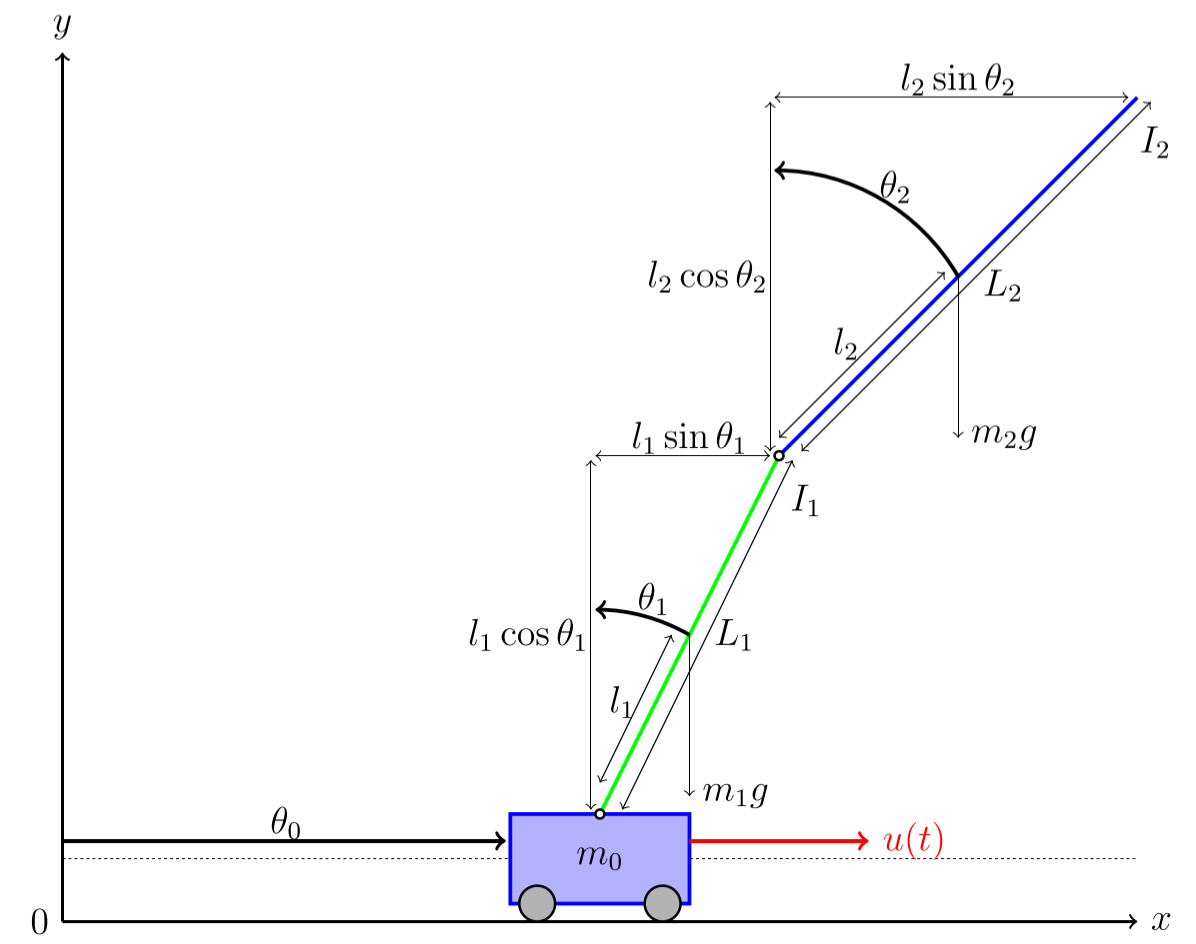
\includegraphics[width=\linewidth]{../Modelo Teorico/ImagenesModelo Teorico/sistema}
	\caption{Modelo teórico del doble péndulo invertido.}	
	\label{fig:pendteo}
\end{figure}
Luego utilizando la formulación de Euler-Lagrange.
\begin{equation}
  \frac{d}{dt}\frac{\partial L}{\partial \dot{\Theta}} - \frac{\partial L}{\partial \Theta}  = \tau
\end{equation} 
\begin{equation}
L\left( \Theta , \dot{\Theta} \right) = \sum_{i=0}^2
\left( \frac{1}{2} m_i v_{Ci}^Tv_{Ci} +\frac{1}{2} I_i \omega_{Ci}^T\omega_{Ci} + u_{refi} - m_i g d_{Ci}\right)
\end{equation} 
Se llega al sistema de segundo orden no lineal:
\begin{equation}
\tau = M\left( \Theta \right)\ddot{\Theta} + V\left( \Theta , \dot{\Theta} \right) + G\left( \Theta \right)
\end{equation}
Siendo las matrices:
\begin{equation}
 M\left( \Theta \right)\ddot{\Theta} = \begin{bmatrix}
m_0+m_1+m_2 & \left( m_1l_1 + m_2L_1 \right) \cos \theta_1 & m_2l_2 \cos \theta_2\\

\left( m_1l_1 + m_2L_1 \right) \cos \theta_1  &
m_1l_1^2+m_2L_1^2+I_1
& m_2L_1l_2\cos(\theta_1-\theta_2)\\


m_2l_2\cos\theta_2 & m_2L_1l_2\cos(\theta_1-\theta_2) & m_2l_2^2+I_2
\end{bmatrix}
\end{equation}
\begin{equation}
 V\left( \Theta , \dot{\Theta} \right) =
 \begin{bmatrix}
0 & -\left( m_1l_1 + m_2L_1 \right)\sin \theta_1 \dot{\theta_1} & -m_2l_2\sin \theta_2 \dot{\theta_2}\\
0 & 0 & m_2L_1l_2\sin(\theta_1-\theta_2)\dot{\theta_2}\\
0 & -m_2L_1l_2\sin(\theta_1-\theta_2)\dot{\theta_1} & 0
\end{bmatrix}
\end{equation}
\begin{equation}
 G\left( \Theta \right) = \begin{bmatrix}
0 \\
 -(m_1l_1+m_2L_1)g\sin\theta_1 \\
-m_2gl_2\sin\theta_2
\end{bmatrix}
\end{equation}
\begin{equation}
 H = \begin{bmatrix}
1 \\
 0 \\
0
\end{bmatrix}
\hspace{1cm}
\tau = H\cdot u(t)
\end{equation}
Si se asume los siguientes valores:
\begin{equation}
l1 = \frac{1}{2} L_1
\hspace{1cm}
l2 = \frac{1}{2} L_2 
\hspace{1cm}
I_1 = \frac{1}{12} m_1L_1^2
\hspace{1cm}
I_2 = \frac{1}{12} m_2L_2^2
\end{equation}
Se simplifica a :
\begin{equation}
 M\left( \Theta \right)\ddot{\Theta} = \begin{bmatrix}
m_0+m_1+m_2 & \left( \frac{1}{2}m_1L_1 + m_2 \right) L_1\cos \theta_1  \frac{1}{2}& m_2L_2 \cos \theta_2\\

\left(  \frac{1}{2}m_1 + m_2 \right) L_1 \cos \theta_1  &
\left( \frac{1}{3}m_1+m_2\right) L_1^2
&  \frac{1}{2}m_2L_1L_2\cos(\theta_1-\theta_2)\\


 \frac{1}{2}m_2L_2\cos\theta_2 &  \frac{1}{2}m_2L_1L_2\cos(\theta_1-\theta_2) &  \frac{1}{3}m_2L_2^2
\end{bmatrix}
\end{equation}
\begin{equation}
 V\left( \Theta , \dot{\Theta} \right) =
 \begin{bmatrix}
0 & -\left(  \frac{1}{2}m_1 + m_2\right)L_1\sin \theta_1 \dot{\theta_1} & - \frac{1}{2}m_2L_2\sin \theta_2 \dot{\theta_2}\\
0 & 0 &  \frac{1}{2}m_2L_1L_2\sin(\theta_1-\theta_2)\dot{\theta_2}\\
0 & - \frac{1}{2}m_2L_1L_2\sin(\theta_1-\theta_2)\dot{\theta_1} & 0
\end{bmatrix}
\end{equation}
\begin{equation}
 G\left( \Theta \right) = \begin{bmatrix}
0 \\
 - \frac{1}{2}(m_1+m_2)L_1g\sin\theta_1 \\
- \frac{1}{2}m_2gL_2\sin\theta_2
\end{bmatrix}
\end{equation}
\begin{equation}
 H = \begin{bmatrix}
1 \\
 0 \\
0
\end{bmatrix}
\hspace{1cm}
\tau = H\cdot u(t)
\end{equation}
Cabe mencionar que $M(\Theta)$ es una matriz simétrica no-singular, por lo que existe la inversa y también es simétrica.

%\end{document}

\Section{Simulación}
\label{sec:simulacion}
%\documentclass[a4paper]{article}
\usepackage[utf8]{inputenc}
\usepackage[spanish, es-tabla, es-noshorthands]{babel}
\usepackage[table,xcdraw]{xcolor}
\usepackage[a4paper, footnotesep=1.25cm, headheight=1.25cm, top=2.54cm, left=2.54cm, bottom=2.54cm, right=2.54cm]{geometry}
%\geometry{showframe}

%\usepackage{wrapfig}			%Wrap figure in text
\usepackage[export]{adjustbox}	%Move images
\usepackage{changepage}			%Move tables

\usepackage{tikz}
\usepackage{amsmath}
\usepackage{amsfonts}
\usepackage{amssymb}
\usepackage{float}
\usepackage{graphicx}
\usepackage{caption}
\usepackage{subcaption}
\usepackage{multicol}
\usepackage{multirow}
\usepackage{wrapfig}
\setlength{\doublerulesep}{\arrayrulewidth}
\usepackage{booktabs}
\usepackage[numbib, nottoc, notlot, notlof]{tocbibind}

\usepackage{hyperref}
\hypersetup{
    colorlinks=true,
    linkcolor=blue,
    filecolor=magenta,      
    urlcolor=blue,
    citecolor=blue,    
}

%Change Font Size

% #1 = size, #2 = text
\newcommand{\setparagraphsize}[2]{{\fontsize{#1}{6}\selectfont#2 \par}}		%Cambia el size de todo el parrafo
\newcommand{\setlinesize}[2]{{\fontsize{#1}{6}\selectfont#2}}				%Cambia el font de una oración

\newcommand{\note}[1]{
	\begin{center}
		\huge{ \textcolor{red}{#1} }
	\end{center}
}

%FONTS (IMPORTANTE): Compilar en XeLaTex o LuaLaTeX
\usepackage{anyfontsize}	%Font size
\usepackage{fontspec}		%Font type

\usepackage{etoolbox}
\usepackage{todonotes}

\newcommand{\observacion}[2]{  \ifnumequal{1}{#1}{ { \todo[inline,backgroundcolor=red!25,bordercolor=red!100]{\textbf{Observación: #2}} } }{  }  }

\setcounter{topnumber}{2}
\setcounter{bottomnumber}{2}
\setcounter{totalnumber}{4}
\renewcommand{\topfraction}{0.85}
\renewcommand{\bottomfraction}{0.85}
\renewcommand{\textfraction}{0.15}
\renewcommand{\floatpagefraction}{0.8}
\renewcommand{\textfraction}{0.1}
\setlength{\floatsep}{5pt plus 2pt minus 2pt}
\setlength{\textfloatsep}{5pt plus 2pt minus 2pt}
\setlength{\intextsep}{5pt plus 2pt minus 2pt}

\newcommand{\quotes}[1]{``#1''}
\usepackage{array}
\newcolumntype{C}[1]{>{\centering\let\newline\\\arraybackslash\hspace{0pt}}m{#1}}
\usepackage[american]{circuitikz}
\usetikzlibrary{calc}
\usepackage{fancyhdr}
\usepackage{units} 

\graphicspath{{../Control de posición no lineal/}{../Control de fuerza no lineal/}{../Control híbrido no lineal/}{../Referencias/}{../Deducción de modelo/}{../Conclusiones/}}

\pagestyle{fancy}
\fancyhf{}
\lhead{22.99 - Automación Industrial}
\rhead{Lambertucci, Londero B., Maselli, Mechoulam}
\rfoot{Página \thepage}

%Items con bullets y no cuadrados
\renewcommand{\labelitemi}{\textbullet }

%
%\begin{document}

\Subsection{Modelo de Simscape}
\Subsection{Simulink}
%\end{document}
\Section{Modelo de Control}
\label{sec:modelodecontrol}
%\documentclass[a4paper]{article}
\usepackage[utf8]{inputenc}
\usepackage[spanish, es-tabla, es-noshorthands]{babel}
\usepackage[table,xcdraw]{xcolor}
\usepackage[a4paper, footnotesep=1.25cm, headheight=1.25cm, top=2.54cm, left=2.54cm, bottom=2.54cm, right=2.54cm]{geometry}
%\geometry{showframe}

%\usepackage{wrapfig}			%Wrap figure in text
\usepackage[export]{adjustbox}	%Move images
\usepackage{changepage}			%Move tables

\usepackage{tikz}
\usepackage{amsmath}
\usepackage{amsfonts}
\usepackage{amssymb}
\usepackage{float}
\usepackage{graphicx}
\usepackage{caption}
\usepackage{subcaption}
\usepackage{multicol}
\usepackage{multirow}
\usepackage{wrapfig}
\setlength{\doublerulesep}{\arrayrulewidth}
\usepackage{booktabs}
\usepackage[numbib, nottoc, notlot, notlof]{tocbibind}

\usepackage{hyperref}
\hypersetup{
    colorlinks=true,
    linkcolor=blue,
    filecolor=magenta,      
    urlcolor=blue,
    citecolor=blue,    
}

%Change Font Size

% #1 = size, #2 = text
\newcommand{\setparagraphsize}[2]{{\fontsize{#1}{6}\selectfont#2 \par}}		%Cambia el size de todo el parrafo
\newcommand{\setlinesize}[2]{{\fontsize{#1}{6}\selectfont#2}}				%Cambia el font de una oración

\newcommand{\note}[1]{
	\begin{center}
		\huge{ \textcolor{red}{#1} }
	\end{center}
}

%FONTS (IMPORTANTE): Compilar en XeLaTex o LuaLaTeX
\usepackage{anyfontsize}	%Font size
\usepackage{fontspec}		%Font type

\usepackage{etoolbox}
\usepackage{todonotes}

\newcommand{\observacion}[2]{  \ifnumequal{1}{#1}{ { \todo[inline,backgroundcolor=red!25,bordercolor=red!100]{\textbf{Observación: #2}} } }{  }  }

\setcounter{topnumber}{2}
\setcounter{bottomnumber}{2}
\setcounter{totalnumber}{4}
\renewcommand{\topfraction}{0.85}
\renewcommand{\bottomfraction}{0.85}
\renewcommand{\textfraction}{0.15}
\renewcommand{\floatpagefraction}{0.8}
\renewcommand{\textfraction}{0.1}
\setlength{\floatsep}{5pt plus 2pt minus 2pt}
\setlength{\textfloatsep}{5pt plus 2pt minus 2pt}
\setlength{\intextsep}{5pt plus 2pt minus 2pt}

\newcommand{\quotes}[1]{``#1''}
\usepackage{array}
\newcolumntype{C}[1]{>{\centering\let\newline\\\arraybackslash\hspace{0pt}}m{#1}}
\usepackage[american]{circuitikz}
\usetikzlibrary{calc}
\usepackage{fancyhdr}
\usepackage{units} 

\graphicspath{{../Control de posición no lineal/}{../Control de fuerza no lineal/}{../Control híbrido no lineal/}{../Referencias/}{../Deducción de modelo/}{../Conclusiones/}}

\pagestyle{fancy}
\fancyhf{}
\lhead{22.99 - Automación Industrial}
\rhead{Lambertucci, Londero B., Maselli, Mechoulam}
\rfoot{Página \thepage}

%Items con bullets y no cuadrados
\renewcommand{\labelitemi}{\textbullet }

%%
%\begin{document}


\Subsection{Realimentaci\'on de Estados}

Partiendo del sistema con fricción de la simulación, se comprueba la controlabilidad de este de manera homóloga a la explicada en la Sección (\ref{sec:ctrbyobsv}). 




Luego, se realizó la realimentación de estados utilizando el comando \textit{place} de Matlab, colocando a los polos según la Tabla (\ref{tab:realim}).

\begin{table}[H]
\centering
\begin{tabular}{@{}cccccc@{}}
\toprule
\multicolumn{6}{c}{Posición de los Polos} \\ \midrule
-3   & -2.5   & -2.4  & -2  & -1.9  & -1.8  \\ \bottomrule
\end{tabular}
\end{table}
\label{tab:realim}

La posición de los polos fue seleccionada de manera tal que el control sea rápido, pero no lo suficientemente rápido como para que la entrada no desvíe demasiado al sistema del punto de trabajo, lo cual haría que este se desestabilice ya que se está utilizando una técnica de control lineal en un sistema intrínsecamente no lineal.
Quedando entonces las ganancias de realimentación de la siguiente manera

\begin{table}[H]
\centering
\begin{tabular}{@{}cccccc@{}}
\toprule
\multicolumn{6}{c}{Ganancias}                    \\ \midrule
2.63 & 20.81 & 517.25 & 7.36 & 74.88 & 94.07 \\ \bottomrule
\end{tabular}
\end{table}
Se puede observar que el valor de las ganancias para el realimentador son relativamente bajas, por lo que su implementación en un dsp es mas sencillo.
Se puede observar en la Figura (\ref{fig:realim}) la simulación en bloques implementada en Simulink.

\begin{figure}[H]
	\centering
	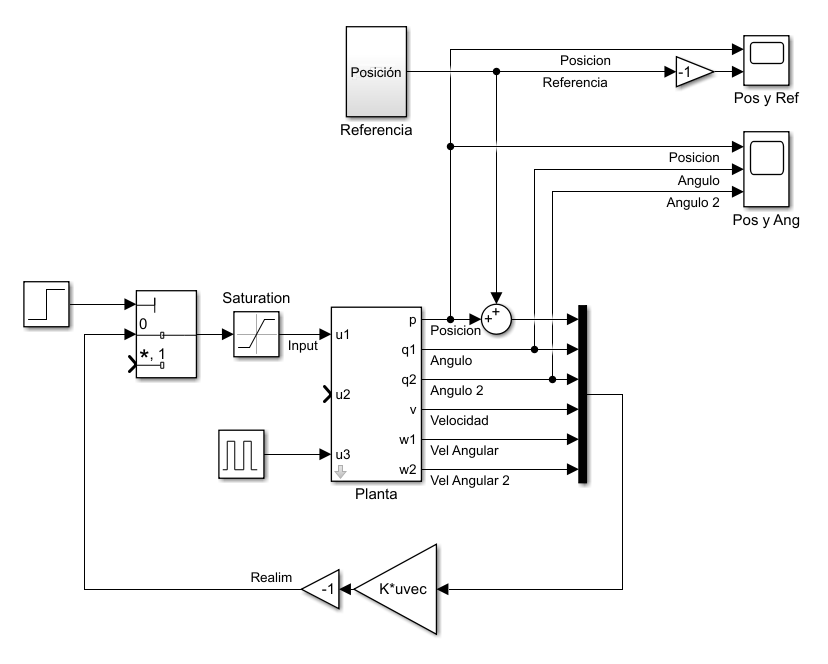
\includegraphics[width=\linewidth]{../Modelo de Control/ImagenesModelo de Control/realim.png}
	\caption{Simulación en bloques de la realimentación de estados.}	
	\label{fig:realim}
\end{figure}

\Subsection{Observador}

Como paso siguiente, se implementó una realimentación de estados con observador. Para esto, se comprobó la observabilidad del sistema con fricción, midiendo la posición del carrito y ambas posiciones angulares para estimar las variables del sistema restantes.

Se decidió colocar los polos del observador de manera tal que estos sean mucho más rápidos que los del sistema. Esto es para que la señal error entre las variables de estado y las estimaciones del observador converga rápidamente a cero. De esta manera, quedaron los polos del observador colocados según la Tabla (\ref{tab:obsv}).

\begin{table}[H]
\centering
\begin{tabular}{@{}cccccc@{}}
\toprule
\multicolumn{6}{c}{Posición de los Polos del Observador} \\ \midrule
-30    & -25    & -24    & -20    & -19    & -18   \\ \bottomrule
\end{tabular}
\end{table}
\label{tab:obsv}

por lo que las ganancias del observador quedan

\begin{table}[H]
\centering
\begin{tabular}{@{}cccccc@{}}
\toprule
\multicolumn{6}{c}{Ganancias}                    \\ \midrule
47.18 & 3.05  & 0.88  & 528.29 & 60.25  & 18.75  \\
2.16  & 43.35 & 0.73  & 40     & 468.40 & 12.29  \\
0.40  & 0.80  & 43.02 & 6.67   & 22.13  & 450.94 \\ \bottomrule
\end{tabular}
\end{table}
Cabe destacar que el valor de las ganancias para el observador son relativamente bajas, por lo que su implementación en un dsp es mas sencillo.

Se puede observar en la Figura (\ref{fig:obsv}) la simulación en bloques implementada en Simulink.

\begin{figure}[H]
	\centering
	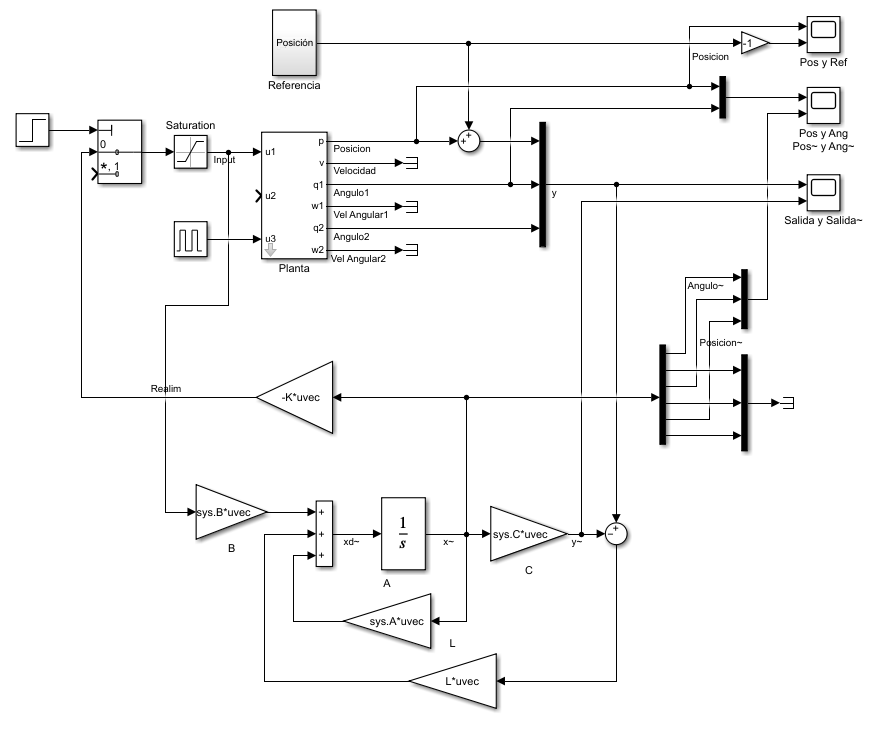
\includegraphics[width=\linewidth]{../Modelo de Control/ImagenesModelo de Control/obsv.png}
	\caption{Simulación en bloques de la realimentación de estados con observador.}	
	\label{fig:obsv}
\end{figure}

\Subsection{Discretizaci\'on}

Como último paso, se decidió pasar a tiempo discreto el sistema original con fricción utilizando la aproximación de Tustin con una tasa de muestreo de $30 \ ms$. Así quedando

\begin{equation}
 A = \begin{bmatrix}
1 &  -0.0010  & 0.0001 & 0.0250 &  0      & 0\\
0 &  1.0051  & -0.0040 & 0     &  0.0249 & 0.0002\\
0 &  -0.0062 & 1.0109  & 0     &  0.0002 & 0.0245\\
0 &  -0.0790  & 0.0092 & 1     &  0.0004 & -0.0015\\
0 &  0.4114  & -0.3190 & 0     &  0.9938 & 0.0173\\
0 &  -0.4971 & 0.8714 & 0     &  0.0151 & 0.9624
\end{bmatrix}
\end{equation}
\begin{equation}
 B = \begin{bmatrix}
0.0001 \\
-0.0001 \\
0.0001 \\
0.0047 \\
-0.0060 \\
0.0072
\end{bmatrix}
\end{equation}
\begin{equation}
 C = \begin{bmatrix}
1 &  -0.0005  & 0.0001 & 0.0125 &  0      & 0\\
0 &  1.0026  & -0.0020 & 0     &  0.0125 & 0.0001\\
0 &  -0.0031 & 1.0054  & 0     &  0.0001 & 0.0123
\end{bmatrix}
\end{equation}
\begin{equation}
 D = \begin{bmatrix}
0.2952 \cdot 10^{-4} \\
-0.3748 \cdot 10^{-4} \\
0.4529  \cdot 10^{-4}
\end{bmatrix}
\end{equation}

para luego realizar la realimentación de estados con observador, midiendo la posición del carrito y las posiciones angulares. Los polos se colocaron de manera siguiente

\begin{table}[H]
\centering
\begin{tabular}{@{}cccccc@{}}
\toprule
\multicolumn{6}{c}{Posición de los Polos (Plano Z)}                \\ \midrule
0.9560    & 0.9531    & 0.9503    & 0.9418   & 0.9389   & 0.9361   \\ \midrule
\multicolumn{6}{c}{Posición de los Polos del Observador (Plano Z)} \\ \midrule
0.4066    & 0.3829    & 0.3606    & 0.3012   & 0.2837   & 0.2671   \\ \bottomrule
\end{tabular}
\end{table}

quedando las ganancias de realimentación

\begin{table}[H]
\centering
\begin{tabular}{@{}clllll@{}}
\toprule
\multicolumn{6}{c}{Ganancias de Realimentación}                           \\ \midrule
0.7006 & \multicolumn{1}{c}{-34.1842} & \multicolumn{1}{c}{339.4479} & \multicolumn{1}{c}{2.3704}  & \multicolumn{1}{c}{34.6514} & \multicolumn{1}{c}{56.0334} \\ \midrule
\multicolumn{6}{c}{Ganancias de Realimentación del Observador}            \\ \midrule
1.4308 & \multicolumn{1}{c}{0.0081}   & \multicolumn{1}{c}{0.0018}   & \multicolumn{1}{c}{28.9658} & \multicolumn{1}{c}{0.4876}  & \multicolumn{1}{c}{0.1119}  \\
\multicolumn{1}{l}{0.0061} & 1.4318 & 0.0063 & 0.3489 & 29.0873 & 0.4613  \\
\multicolumn{1}{l}{0.0007} & 0.0071 & 1.4153 & 0.0161 & 0.6202  & 27.7099 \\ \bottomrule
\end{tabular}
\end{table}
Aquí las ganancias varían entre $10^2$ y $10^-4$ por lo que el realizar cuentas con estos en un dsp resulta sencillo.
Se puede observar en la Figura (\ref{fig:obsv_disc}) la simulación en bloques implementada en Simulink.

\begin{figure}[H]
	\centering
	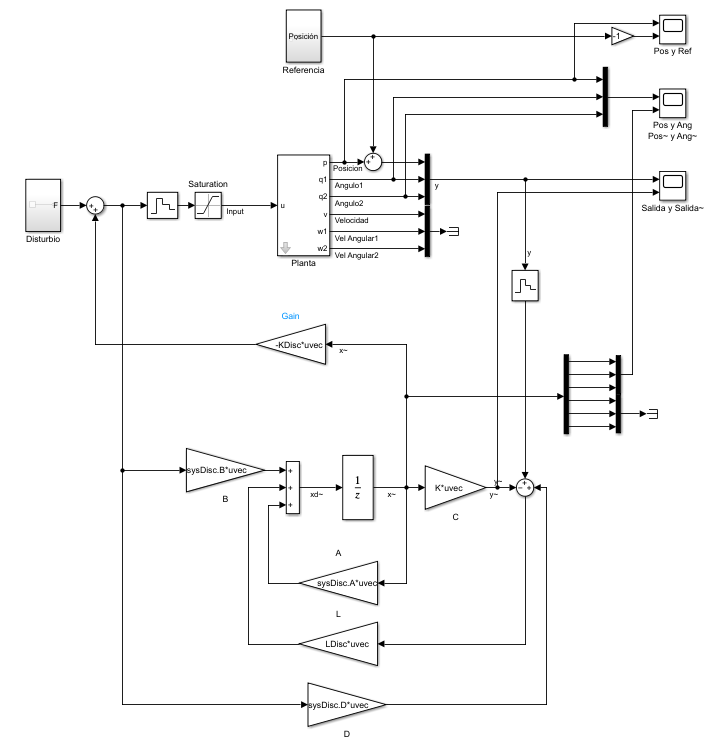
\includegraphics[width=\linewidth]{../Modelo de Control/ImagenesModelo de Control/obsv_disc.png}
	\caption{Simulación en bloques de la realimentación de estados con observador discreto.}	
	\label{fig:obsv_disc}
\end{figure}

\Subsection{Integral}

PENDIENTE

%\end{document}
\Section{An\'alisis de Resultados}
\label{sec:analisisderesultados}
%\documentclass[a4paper]{article}
\usepackage[utf8]{inputenc}
\usepackage[spanish, es-tabla, es-noshorthands]{babel}
\usepackage[table,xcdraw]{xcolor}
\usepackage[a4paper, footnotesep=1.25cm, headheight=1.25cm, top=2.54cm, left=2.54cm, bottom=2.54cm, right=2.54cm]{geometry}
%\geometry{showframe}

%\usepackage{wrapfig}			%Wrap figure in text
\usepackage[export]{adjustbox}	%Move images
\usepackage{changepage}			%Move tables

\usepackage{tikz}
\usepackage{amsmath}
\usepackage{amsfonts}
\usepackage{amssymb}
\usepackage{float}
\usepackage{graphicx}
\usepackage{caption}
\usepackage{subcaption}
\usepackage{multicol}
\usepackage{multirow}
\usepackage{wrapfig}
\setlength{\doublerulesep}{\arrayrulewidth}
\usepackage{booktabs}
\usepackage[numbib, nottoc, notlot, notlof]{tocbibind}

\usepackage{hyperref}
\hypersetup{
    colorlinks=true,
    linkcolor=blue,
    filecolor=magenta,      
    urlcolor=blue,
    citecolor=blue,    
}

%Change Font Size

% #1 = size, #2 = text
\newcommand{\setparagraphsize}[2]{{\fontsize{#1}{6}\selectfont#2 \par}}		%Cambia el size de todo el parrafo
\newcommand{\setlinesize}[2]{{\fontsize{#1}{6}\selectfont#2}}				%Cambia el font de una oración

\newcommand{\note}[1]{
	\begin{center}
		\huge{ \textcolor{red}{#1} }
	\end{center}
}

%FONTS (IMPORTANTE): Compilar en XeLaTex o LuaLaTeX
\usepackage{anyfontsize}	%Font size
\usepackage{fontspec}		%Font type

\usepackage{etoolbox}
\usepackage{todonotes}

\newcommand{\observacion}[2]{  \ifnumequal{1}{#1}{ { \todo[inline,backgroundcolor=red!25,bordercolor=red!100]{\textbf{Observación: #2}} } }{  }  }

\setcounter{topnumber}{2}
\setcounter{bottomnumber}{2}
\setcounter{totalnumber}{4}
\renewcommand{\topfraction}{0.85}
\renewcommand{\bottomfraction}{0.85}
\renewcommand{\textfraction}{0.15}
\renewcommand{\floatpagefraction}{0.8}
\renewcommand{\textfraction}{0.1}
\setlength{\floatsep}{5pt plus 2pt minus 2pt}
\setlength{\textfloatsep}{5pt plus 2pt minus 2pt}
\setlength{\intextsep}{5pt plus 2pt minus 2pt}

\newcommand{\quotes}[1]{``#1''}
\usepackage{array}
\newcolumntype{C}[1]{>{\centering\let\newline\\\arraybackslash\hspace{0pt}}m{#1}}
\usepackage[american]{circuitikz}
\usetikzlibrary{calc}
\usepackage{fancyhdr}
\usepackage{units} 

\graphicspath{{../Control de posición no lineal/}{../Control de fuerza no lineal/}{../Control híbrido no lineal/}{../Referencias/}{../Deducción de modelo/}{../Conclusiones/}}

\pagestyle{fancy}
\fancyhf{}
\lhead{22.99 - Automación Industrial}
\rhead{Lambertucci, Londero B., Maselli, Mechoulam}
\rfoot{Página \thepage}

%Items con bullets y no cuadrados
\renewcommand{\labelitemi}{\textbullet }

%
%\begin{document}
\Subsection{Realimentación de Estados}
%\end{document}
\newpage
\Section{Conclusiones}
\label{sec:conclusiones}
%\documentclass[a4paper]{article}
\usepackage[utf8]{inputenc}
\usepackage[spanish, es-tabla, es-noshorthands]{babel}
\usepackage[table,xcdraw]{xcolor}
\usepackage[a4paper, footnotesep=1.25cm, headheight=1.25cm, top=2.54cm, left=2.54cm, bottom=2.54cm, right=2.54cm]{geometry}
%\geometry{showframe}

%\usepackage{wrapfig}			%Wrap figure in text
\usepackage[export]{adjustbox}	%Move images
\usepackage{changepage}			%Move tables

\usepackage{tikz}
\usepackage{amsmath}
\usepackage{amsfonts}
\usepackage{amssymb}
\usepackage{float}
\usepackage{graphicx}
\usepackage{caption}
\usepackage{subcaption}
\usepackage{multicol}
\usepackage{multirow}
\usepackage{wrapfig}
\setlength{\doublerulesep}{\arrayrulewidth}
\usepackage{booktabs}
\usepackage[numbib, nottoc, notlot, notlof]{tocbibind}

\usepackage{hyperref}
\hypersetup{
    colorlinks=true,
    linkcolor=blue,
    filecolor=magenta,      
    urlcolor=blue,
    citecolor=blue,    
}

%Change Font Size

% #1 = size, #2 = text
\newcommand{\setparagraphsize}[2]{{\fontsize{#1}{6}\selectfont#2 \par}}		%Cambia el size de todo el parrafo
\newcommand{\setlinesize}[2]{{\fontsize{#1}{6}\selectfont#2}}				%Cambia el font de una oración

\newcommand{\note}[1]{
	\begin{center}
		\huge{ \textcolor{red}{#1} }
	\end{center}
}

%FONTS (IMPORTANTE): Compilar en XeLaTex o LuaLaTeX
\usepackage{anyfontsize}	%Font size
\usepackage{fontspec}		%Font type

\usepackage{etoolbox}
\usepackage{todonotes}

\newcommand{\observacion}[2]{  \ifnumequal{1}{#1}{ { \todo[inline,backgroundcolor=red!25,bordercolor=red!100]{\textbf{Observación: #2}} } }{  }  }

\setcounter{topnumber}{2}
\setcounter{bottomnumber}{2}
\setcounter{totalnumber}{4}
\renewcommand{\topfraction}{0.85}
\renewcommand{\bottomfraction}{0.85}
\renewcommand{\textfraction}{0.15}
\renewcommand{\floatpagefraction}{0.8}
\renewcommand{\textfraction}{0.1}
\setlength{\floatsep}{5pt plus 2pt minus 2pt}
\setlength{\textfloatsep}{5pt plus 2pt minus 2pt}
\setlength{\intextsep}{5pt plus 2pt minus 2pt}

\newcommand{\quotes}[1]{``#1''}
\usepackage{array}
\newcolumntype{C}[1]{>{\centering\let\newline\\\arraybackslash\hspace{0pt}}m{#1}}
\usepackage[american]{circuitikz}
\usetikzlibrary{calc}
\usepackage{fancyhdr}
\usepackage{units} 

\graphicspath{{../Control de posición no lineal/}{../Control de fuerza no lineal/}{../Control híbrido no lineal/}{../Referencias/}{../Deducción de modelo/}{../Conclusiones/}}

\pagestyle{fancy}
\fancyhf{}
\lhead{22.99 - Automación Industrial}
\rhead{Lambertucci, Londero B., Maselli, Mechoulam}
\rfoot{Página \thepage}

%Items con bullets y no cuadrados
\renewcommand{\labelitemi}{\textbullet }

%
%\begin{document}

Se tuvo la oportunidad de desarrollar analíticamente la mecánica del manipulador propuesto por la cátedra, obteniendo a través del método de Lagrange el vector de torques, al igual que por propagación de velocidades la matriz jacobiana. Se llevaron adelante diversos tipos de control, tanto de posición y fuerzo e incluso uno híbrido, el cual incluye ambas variables mencioandas.

Se exploraron varias topologías de control no lineal, como puede ser la linealización por punto de equilibrio variable y la linealización por realimentación. La utilizada fue la linealización por realimentación debido al amplio conocimiento que se tiene sobre la planta. 

Se profundizó en el uso de simulink, al igual que un aprendizaje en el uso del toolbox de robotics de Peter Corke, herramienta para la simulación de manipuladores. 

Finalmente se observó la reacción de los distintos tipos de control ante disturbios en la planta, y como estos vuelven a sus señales respectivas de referencia.

%\end{document}

	

\documentclass[a4paper]{article}
\usepackage[utf8]{inputenc}
\usepackage[spanish, es-tabla, es-noshorthands]{babel}
\usepackage[table,xcdraw]{xcolor}
\usepackage[a4paper, footnotesep=1.25cm, headheight=1.25cm, top=2.54cm, left=2.54cm, bottom=2.54cm, right=2.54cm]{geometry}
%\geometry{showframe}

%\usepackage{wrapfig}			%Wrap figure in text
\usepackage[export]{adjustbox}	%Move images
\usepackage{changepage}			%Move tables

\usepackage{tikz}
\usepackage{amsmath}
\usepackage{amsfonts}
\usepackage{amssymb}
\usepackage{float}
\usepackage{graphicx}
\usepackage{caption}
\usepackage{subcaption}
\usepackage{multicol}
\usepackage{multirow}
\usepackage{wrapfig}
\setlength{\doublerulesep}{\arrayrulewidth}
\usepackage{booktabs}
\usepackage[numbib, nottoc, notlot, notlof]{tocbibind}

\usepackage{hyperref}
\hypersetup{
    colorlinks=true,
    linkcolor=blue,
    filecolor=magenta,      
    urlcolor=blue,
    citecolor=blue,    
}

%Change Font Size

% #1 = size, #2 = text
\newcommand{\setparagraphsize}[2]{{\fontsize{#1}{6}\selectfont#2 \par}}		%Cambia el size de todo el parrafo
\newcommand{\setlinesize}[2]{{\fontsize{#1}{6}\selectfont#2}}				%Cambia el font de una oración

\newcommand{\note}[1]{
	\begin{center}
		\huge{ \textcolor{red}{#1} }
	\end{center}
}

%FONTS (IMPORTANTE): Compilar en XeLaTex o LuaLaTeX
\usepackage{anyfontsize}	%Font size
\usepackage{fontspec}		%Font type

\usepackage{etoolbox}
\usepackage{todonotes}

\newcommand{\observacion}[2]{  \ifnumequal{1}{#1}{ { \todo[inline,backgroundcolor=red!25,bordercolor=red!100]{\textbf{Observación: #2}} } }{  }  }

\setcounter{topnumber}{2}
\setcounter{bottomnumber}{2}
\setcounter{totalnumber}{4}
\renewcommand{\topfraction}{0.85}
\renewcommand{\bottomfraction}{0.85}
\renewcommand{\textfraction}{0.15}
\renewcommand{\floatpagefraction}{0.8}
\renewcommand{\textfraction}{0.1}
\setlength{\floatsep}{5pt plus 2pt minus 2pt}
\setlength{\textfloatsep}{5pt plus 2pt minus 2pt}
\setlength{\intextsep}{5pt plus 2pt minus 2pt}

\newcommand{\quotes}[1]{``#1''}
\usepackage{array}
\newcolumntype{C}[1]{>{\centering\let\newline\\\arraybackslash\hspace{0pt}}m{#1}}
\usepackage[american]{circuitikz}
\usetikzlibrary{calc}
\usepackage{fancyhdr}
\usepackage{units} 

\graphicspath{{../Control de posición no lineal/}{../Control de fuerza no lineal/}{../Control híbrido no lineal/}{../Referencias/}{../Deducción de modelo/}{../Conclusiones/}}

\pagestyle{fancy}
\fancyhf{}
\lhead{22.99 - Automación Industrial}
\rhead{Lambertucci, Londero B., Maselli, Mechoulam}
\rfoot{Página \thepage}

%Items con bullets y no cuadrados
\renewcommand{\labelitemi}{\textbullet }


\begin{document}

\begin{flushleft}
\begin{thebibliography}{9}

\bibitem{ref:final}
\quotes{Limit switch - Wikipedia}, En.wikipedia.org, 2021. [Online]. Disponible: \href{https://en.wikipedia.org/wiki/Limit\_switch}{https://en.wikipedia.org/wiki/Limit\_switch}. [Accedido: 28 Agosto 2021].

\end{thebibliography}
\end{flushleft}

\end{document}


\end{document}